\section{METODOLOGI}

% Ubah konten-konten berikut sesuai dengan isi dari metodologi

\subsection{Data dan Peralatan/ Data dan Alat Bantu/ Material }

% Berikut merupakan data dan perlatan yang mendukung pengerjaan Tugas Akhir ini.
\begin{itemize}
   \item [$\bullet$]Dataset berupa gambar bangun datar segitiga, persegi, persegi panjang, lingkaran, dan trapesium berjumlah 50 gambar untuk tiap bangun datar
   
    % \begin{figure} [H] \centering
    %   % Nama dari file gambar yang diinputkan
    %   \includegraphics[scale=0.2]{gambar/UTKFace.png}
    %   % Keterangan gambar yang diinputkan
    %   \caption{Dataset UTKFace}
    %   % Label referensi dari gambar yang diinputkan
    %   \label{fig:UTKFace}
    % \end{figure}

   \item [$\bullet$]Dataset berupa gambar tulisan parameter bangun datar 
    \begin{itemize}
      \item [$\bullet$]Untuk bangun datar segitiga parameternya adalah huruf A(alas) dan T(tinggi) berjumlah 50 gambar untuk tiap huruf
      \item [$\bullet$]Untuk bangun datar persegi parameternya adalah huruf S(sisi) berjumlah 50 gambar untuk tiap huruf
      \item [$\bullet$]Untuk bangun datar persegi panjang parameternya adalah huruf P(panjang) dan L(lebar) berjumlah 50 gambar untuk tiap huruf
      \item [$\bullet$]Untuk bangun datar lingkaran parameternya adalah huruf R(jari-jari) berjumlah 50 gambar untuk tiap huruf
      \item [$\bullet$]Untuk bangun datar trapesium parameternya adalah huruf S1(sisi atas), S2(sisi bawah), dan T(tinggi) berjumlah 50 gambar untuk tiap huruf
      \item [$\bullet$]Angka untuk parameter (1,2,3,4,5,6,7,8,9,0) berjumlah 50 gambar untuk tiap angka
    \end{itemize}

   \item [$\bullet$]Kamera \\
   
\end{itemize}
   

\subsection{Metodologi Penelitian}
% Metodologi yang digunakan dalam pengerjaan Tugas Akhir ini adalah sebagai berikut.
    % Contoh input gambar dengan format *.jpg
    \begin{figure} [H] \centering
      % Nama dari file gambar yang diinputkan
      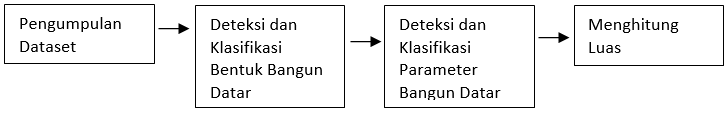
\includegraphics[scale=0.7]{gambar/Metodologi.png}
      % Keterangan gambar yang diinputkan
      \caption{Diagram blok metodologi}
      % Label referensi dari gambar yang diinputkan
      \label{fig:Metodologi}
    \end{figure}

\begin{enumerate}
   \item \textbf{Pengumpulan dataset} \\
   Pengumpulan dataset dilakukan dengan menggambar bangun datar dan parameter bangun datar pada papan tulis lalu disimpan dalam bentuk foto.
   \item \textbf{Deteksi dan Klasifikasi Bentuk Bangun Datar} \\
   Citra diproses dari kamera lalu program akan mendeteksi dan mengklasifikasi bentuk bangun datar
   \item \textbf{Deteksi dan Klasifikasi Parameter Bangun Datar} \\
   Citra diproses dari kamera lalu program akan mendeteksi dan mengklasifikasi parameter bangun datar
   \item \textbf{Menghitung Luas} \\
   Dari hasil deteksi dan klasifikasi, program akan melakukan perhitungan luas sebuah bangun datar
\end{enumerate}